\section{Desafio}
  
A continuación se muestra una forma tentativa del desafío. La clave es darse cuenta que las sumatorias se pueden calcular por separado y operarlas de a poco.

  \lstinputlisting[
    style  = mypy,
    caption= \texttt{desafio.py}]{Code/desafio.py}

Visualmente, una gráfica de lo anterior es
\begin{figure}[h]
    \centering
    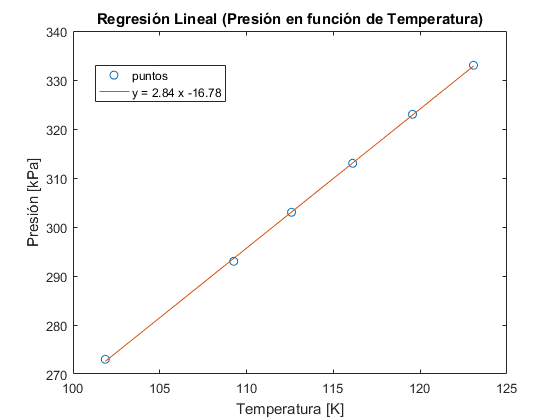
\includegraphics[scale=0.55]{Imagenes/regresion.png}
    \caption{En base a los datos de un experimento, se llega a una expresión general}
\end{figure}